
%(BEGIN_QUESTION)
% Copyright 2006, Tony R. Kuphaldt, released under the Creative Commons Attribution License (v 1.0)
% This means you may do almost anything with this work of mine, so long as you give me proper credit

Complete a table showing $x$ and $y$ values for the following equation, then plot the equation on the coordinate grid provided:

$$y = 3x + 2$$

% No blank lines allowed between lines of an \halign structure!
% I use comments (%) instead, so that TeX doesn't choke.

$$\vbox{\offinterlineskip
\halign{\strut
\vrule \quad\hfil # \ \hfil & 
\vrule \quad\hfil # \ \hfil \vrule \cr
\noalign{\hrule}
%
% First row
$x$ & $y$ \cr
%
\noalign{\hrule}
%
% Another row
-3 &  \cr
%
\noalign{\hrule}
%
% Another row
-2 &  \cr
%
\noalign{\hrule}
%
% Another row
-1 &  \cr
%
\noalign{\hrule}
%
% Another row
0 &  \cr
%
\noalign{\hrule}
%
% Another row
1 &  \cr
%
\noalign{\hrule}
%
% Another row
2 &  \cr
%
\noalign{\hrule}
%
% Another row
3 &  \cr
%
\noalign{\hrule}
} % End of \halign 
}$$ % End of \vbox

$$\includegraphics[width=15.5cm]{i01514x01.eps}$$

Calculate the slope (at any point) for this equation.  Explain both how you may determine the slope by looking at $x$ and $y$ values in the table, and also by examining the written equation.

\underbar{file i01514}
%(END_QUESTION)





%(BEGIN_ANSWER)

Slope = 3

$$\includegraphics[width=15.5cm]{i01514x02.eps}$$

%(END_ANSWER)





%(BEGIN_NOTES)


%INDEX% Mathematics, calculus: slope of a linear function

%(END_NOTES)


